%%% LaTeX Template: Article/Thesis/etc. with colored headings and special fonts
%%%
%%% Source: http://www.howtotex.com/
%%% Feel free to distribute this template, but please keep to referal to http://www.howtotex.com/ here.
%%% February 2011
%%%
%%% Modified January 2016 by CDM

%%%  Preamble
\documentclass[11pt,letterpaper]{article}
\usepackage[margin=1.0in]{geometry}
\usepackage[T1]{fontenc}
\usepackage[bitstream-charter]{mathdesign}
\usepackage[latin1]{inputenc}					
\usepackage{amsmath}						
\usepackage{xcolor}
\usepackage{cite}
\usepackage{hyphenat}
\usepackage{graphicx}
\usepackage{float}
\usepackage{subfigure}
\usepackage{sectsty}
\usepackage[compact]{titlesec} 
\usepackage[tablegrid]{vhistory}
\usepackage{pbox}
\allsectionsfont{\color{accentcolor}\scshape\selectfont}

%%% Definitions
\definecolor{accentcolor}{rgb}{0.0,0.0,0.5} 
\newcommand{\teamname}{Team Gamma}
\newcommand{\productname}{IEEE Robotics Competition}
\newcommand{\coursename}{CSE 4316: Senior Design I}
\newcommand{\semester}{Fall 2021}
\newcommand{\docname}{Architectural Design Specification}
\newcommand{\department}{Department of Computer Science \& Engineering}
\newcommand{\university}{The University of Texas at Arlington}
\newcommand{\authors}{Evan Cornish \\ Kartikey Sharan \\ Zachary Trumbaturi \\ Osama Siddiqui \\ Paola Gonzalez}

%%% Headers and footers
\usepackage{fancyhdr}
	\pagestyle{fancy}						% Enabling the custom headers/footers
\usepackage{lastpage}	
	% Header (empty)
	\lhead{}
	\chead{}
	\rhead{}
	% Footer
	\lfoot{\footnotesize \teamname \ - \semester}
	\cfoot{}
	\rfoot{\footnotesize page \thepage\ of \pageref{LastPage}}	% "Page 1 of 2"
	\renewcommand{\headrulewidth}{0.0pt}
	\renewcommand{\footrulewidth}{0.4pt}

%%% Change the abstract environment
\usepackage[runin]{abstract}			% runin option for a run-in title
%\setlength\absleftindent{30pt}			% left margin
%\setlength\absrightindent{30pt}		% right margin
\abslabeldelim{\quad}	
\setlength{\abstitleskip}{-10pt}
\renewcommand{\abstractname}{}
\renewcommand{\abstracttextfont}{\color{accentcolor} \small \slshape}	% slanted text

%%% Start of the document
\begin{document}

%%% Cover sheet
{\centering \huge \color{accentcolor} \sc \textbf{\department \\ \university} \par}
\vspace{1 in}
{\centering \huge \color{accentcolor} \sc \textbf{\docname \\ \coursename \\ \semester} \par}
\vspace{0.5 in}
\begin{figure}[h!]
	\centering
   	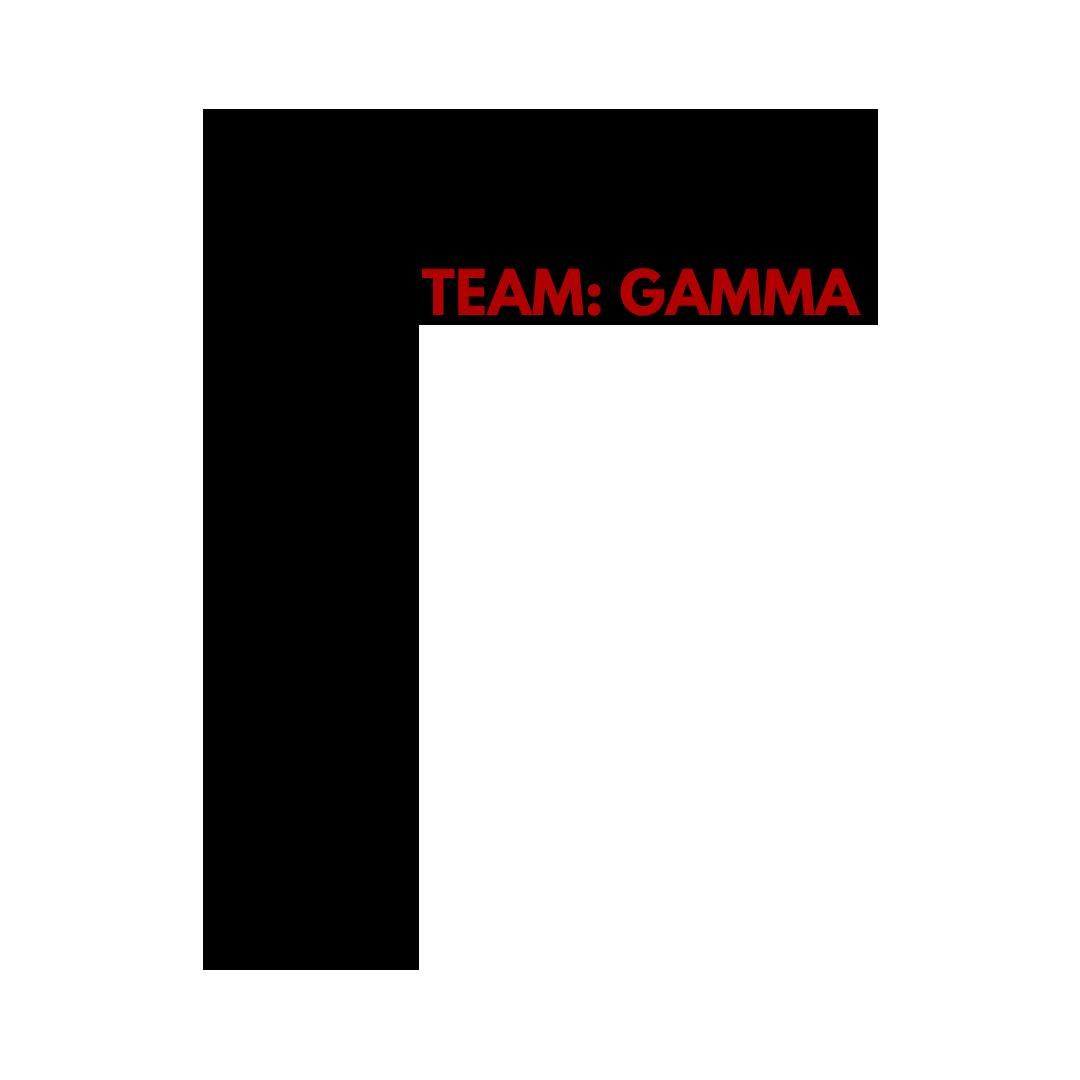
\includegraphics[width=0.60\textwidth]{images/team_gamma}
\end{figure}
\vspace{0.5 in}
{\centering \huge \color{accentcolor} \sc \textbf{\teamname \\ \productname} \par}
\vspace{0.5 in}
{\centering \large \sc \textbf{\authors} \par}
\newpage


%\vspace{1 in}
%\centerline{January 13th, 2012}
%\newpage

%%% Revision History
\begin{versionhistory}
	\vhEntry{0.1}{12.7.2021}{EC|OS|ZT|KS|PG}{document creation}
\end{versionhistory}
\newpage
\newpage

%%% Table of contents
\setcounter{tocdepth}{2}
\tableofcontents
\newpage

%%% List of figures and tables (optional)
\listoffigures
\listoftables
\newpage

%%% Document sections
\section{Introduction}
	This product will be made for the IEEE 2022 robotics competition in Houston Texas on April 2nd. The competition rules explains the full scope of the project but a short summary will be provided here. The objective of the competition is to make a underwater remote controlled submarine that is capable of collecting trash in hard to reach places. As such, the competition includes a number of obstacles that need to be navigated. The submarine will be remote controlled through a series of obstacles that involve hoops both forwards and backwards. Then the robot continues on to the second round. The objective will be to grasp debris that is meant to be mimicking trash in an ocean or river and navigate to a suppository station. The debris will be deposited and then more debris will be collected floating atop the water. That trash will then be deposited in a secondary trash station. In both rounds judges will be watching and award points based on speed, performance, and cost specifications of the robot. The faster and cheaper that the robot can operate the more points will be awarded. 
\newpage
\section{System Overview}
Our submarine design consists of 4 overall design systems. The control system, the movement system, the debris collection system and the visual system. The overall system works together delivering data between these various sub systems in order to insure that the pilot of the submarine can accurately execute actions related to operating the submarine.

\begin{figure}[h!]
	\centering
 	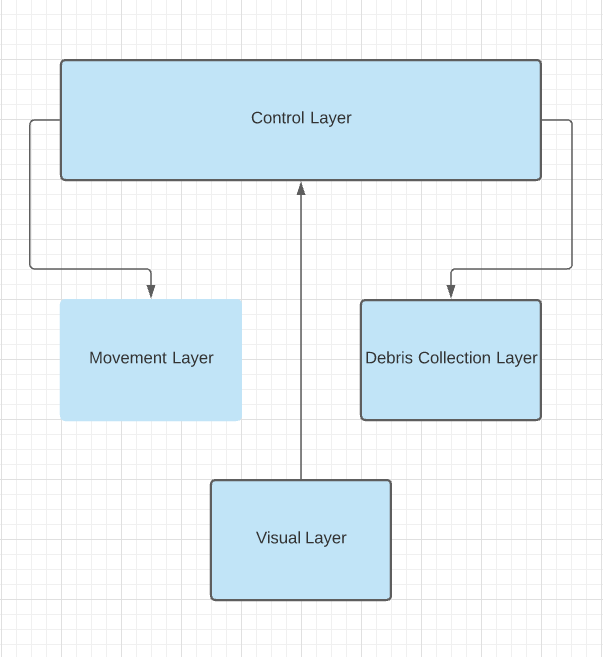
\includegraphics[width=0.60\textwidth]{images/layers}
 \caption{A simple architectural layer diagram}
\end{figure}

\subsection{Control Layer Description}
The control layer involves using the library ArduPilot to call a control system that will operate the underwater vehicle on 6 degrees of freedom. As such the vehicle will need the capability of turning on all axis as well as horizontal spins. It will send its commend through the tether connected to the vehicle and the motor operation will be updated according to the library specifications. The ArduSub sublibrary of the ArduPilot series of libraries has a specification with motor placement that must be followed in order to achieve full functionality from the library.

The control layer also receives input data through the tether from the visual system. That input data is displayed for the pilot onto a monitor system which contains an overlay with some targeting assistance graphics built on top of the display.

All of this data is manipulated through the tether which connects our generic RV controller with micro-controllers installed directly on the vehicle. The vehicle itself will contain between 2-4 micro-controllers that will be responsible for turning on and off the electrical signals.

\subsection{Movement Layer Description}
The movement layer currently consists of a set of 6 thrusters. The thrusters must be placed at predefined specified locations to conform to ArduPilot library's prebuilt specifications. In order to obtain 8 degrees of freedom we will need 2 rear thrusters, and then 4 thrusters placed at various points in a circular fashion all differing by 45 degrees from eachother. The thrusters are turned off and on via electrical signals from micro controllers installed on the vehicle in the control layer. The directional capability of the movement system is all handled automatically by ArduPilot, our system will only implement the thrusters in the specifications according to the ArduPilot library.

\subsection{Debris Collection Layer Description}
The debris collection layer consists of a mechanical arm to collect sunken debris, and a net pulley system to collect floating debris. The net pulley system will collect the floating debris and deposit the debris into a catapult system which will then launch the debris into the collection area. The mechanical arm system will receive signals to clasp the sunken debris from the control system and then release it via the same control system.

\subsection{Visual Layer Description}
The visual layer is the one layer that is meant to deliver information back to the control layer. The information is collected through a waterproof camera on the front of the submarine and then transmitted through the tether to be displayed on the monitor of the control system.  
\newpage
\section{Subsystem Definitions \& Data Flow}

\begin{figure}[h!]
	\centering
 	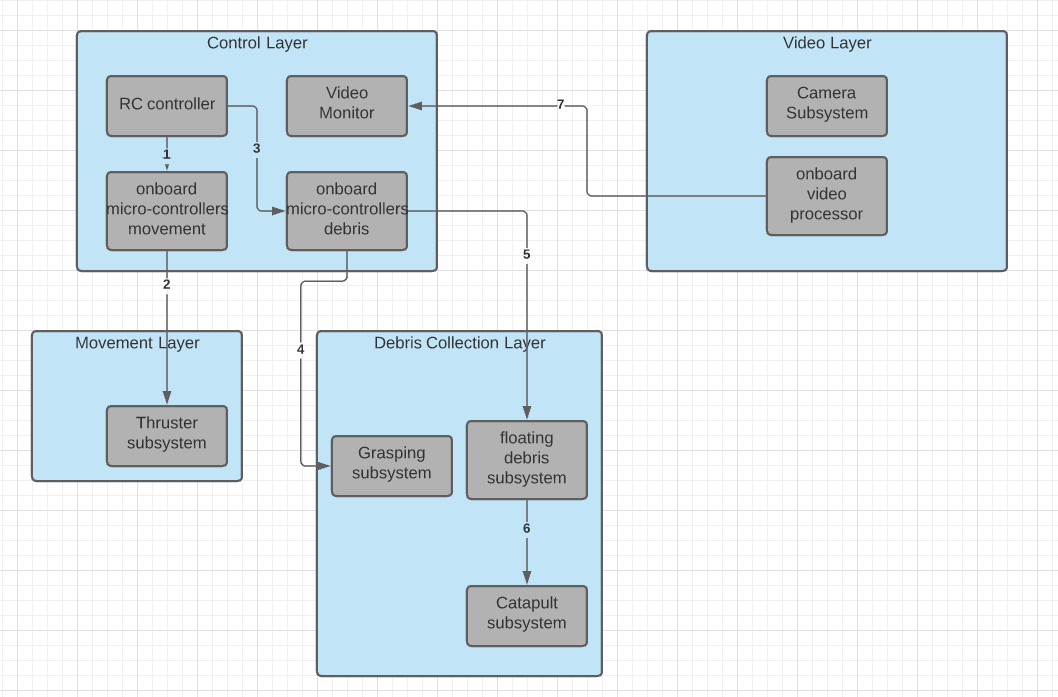
\includegraphics[width=\textwidth]{images/data_flow}
 \caption{A simple data flow diagram}
\end{figure}

\newpage
\section{Control Layer Subsystems}


\subsection{Subsystem 1 RC controller}
We've decided to use a double joystick RC controller for the time being. We have to spend the extra money to buy a remote controller but the benefit would be that the submarine will be easier to pilot. The other option was just using keyboard inputs from a laptop.

\begin{figure}[h!]
	\centering
 	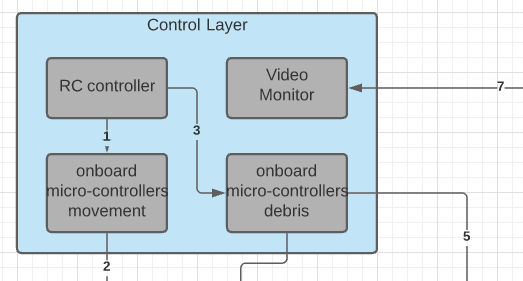
\includegraphics[width=0.60\textwidth]{images/subsystem_control}
 \caption{Example subsystem description diagram}
\end{figure}

\subsubsection{Assumptions}
We made the assumption that easier piloting will lead to higher points. We also assumed that an RC controller is going to be easier to use than keyboard inputs from a laptop.

\subsubsection{Responsibilities}
The responsibilities of the RC controller is to send the electrical signals to the laptop which will then be translated by ArduPilot into actionable instructions on the part of the micro-controllers. 

\subsubsection{Subsystem Interfaces}
Each of the inputs and outputs for the subsystem are defined here. Create a table with an entry for each labelled interface that connects to this subsystem. For each entry, describe any incoming and outgoing data elements will pass through this interface.

\begin {table}[H]
\caption {Subsystem interfaces} 
\begin{center}
    \begin{tabular}{ | p{1cm} | p{6cm} | p{3cm} | p{3cm} |}
    \hline
    ID & Description & Inputs & Outputs \\ \hline
    \#01 & USB interface through tether & \pbox{3cm}{joystick forward backward \\ joystick left-right} & \pbox{3cm}{ArduPilot library calls}  \\ \hline
    \#02 & USB interface & \pbox{3cm}{button clasp} & \pbox{3cm}{micro-controller signal}  \\ \hline
    \end{tabular}
\end{center}
\end{table}

\subsection{Subsystem 2 onboard micro-controllers movement}
\subsubsection{Assumptions}
We've made the assumption that all movement can be controlled by turning power on/off to the thrusters. 

\subsubsection{Responsibilities}
The responsibility is for the micro-controller to give power and/or cut power to the thrusters depending on how we want the submarine to move. The signals for which action the microcontrollers will take will be given via translated library calls from ArduPilot.

\subsubsection{Subsystem Interfaces}

\begin {table}[H]
\caption {Subsystem interfaces} 
\begin{center}
	\begin{tabular}{ | p{1cm} | p{6cm} | p{3cm} | p{3cm} |}
		\hline
		ID & Description & Inputs & Outputs \\ \hline
		\# & USB interface through tether & \pbox{3cm}{USB input} & \pbox{3cm}{Arduino pin signals}  \\ \hline
	\end{tabular}
\end{center}
\end{table}

\subsection{Subsystem 3 onboard micro-controllers debris}
\subsubsection{Assumptions}
we've made the assumption that we will not be able to figure out how to get the arm to clasp without some sort of electrical power solution.

\subsubsection{Responsibilities}
The responsibility of this subsystem is to force the clamp to close when we have the target in sight, and to launch the catapult debris system when it is loaded.

\subsubsection{Subsystem Interfaces}

\begin {table}[H]
\caption {Subsystem interfaces} 
\begin{center}
	\begin{tabular}{ | p{1cm} | p{6cm} | p{3cm} | p{3cm} |}
		\hline
		ID & Description & Inputs & Outputs \\ \hline
		\# & USB interface through tether & \pbox{3cm}{USB input} & \pbox{3cm}{Arduino pin signals}  \\ \hline
	\end{tabular}
\end{center}
\end{table}

\subsection{Subsystem 4 video monitor}
\subsubsection{Assumptions}
we've made the assumption that it will be impossible to pilot the submarine by looking into the water at an angle due to the light reflectivity.

\subsubsection{Responsibilities}
The responsibility of this subsystem is to display the video information being displayed to it from the camera system.

\subsubsection{Subsystem Interfaces}

\begin {table}[H]
\caption {Subsystem interfaces} 
\begin{center}
	\begin{tabular}{ | p{1cm} | p{6cm} | p{3cm} | p{3cm} |}
		\hline
		ID & Description & Inputs & Outputs \\ \hline
		\# & USB interface through tether & \pbox{3cm}{USB input} & \pbox{3cm}{video image}  \\ \hline
	\end{tabular}
\end{center}
\end{table}

\newpage
\section{Movement Layer Subsystems}


\subsection{Subsystem 1 thruster subsystem}

\begin{figure}[h!]
	\centering
 	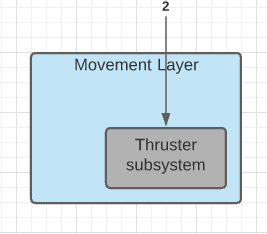
\includegraphics[width=0.60\textwidth]{images/subsystem_movement}
 \caption{Example subsystem description diagram}
\end{figure}

\subsubsection{Assumptions}
We made the assumption that placement of thrusters and general thruster design would be better to copy than to design on our own. We're using our design specifications in accordance with the ArduPilot library documentation.

\subsubsection{Responsibilities}
the responsibility of the thruster subsystem is to move the robot by pushing water through the thrusters. It can also reposition the robot in accordance to the ArduPilot specifications with 8 degrees of freedom.

\subsubsection{Subsystem Interfaces}

\begin {table}[H]
\caption {Subsystem interfaces} 
\begin{center}
    \begin{tabular}{ | p{1cm} | p{6cm} | p{3cm} | p{3cm} |}
    \hline
    ID & Description & Inputs & Outputs \\ \hline
    \#xx & copper wire interface & \pbox{3cm}{electricity} & \pbox{3cm}{kinetic motion}  \\ \hline
    \end{tabular}
\end{center}
\end{table}

\newpage
\section{Debris Layer Subsystems}

\subsection{Subsystem 1 grasping subsystem}

\begin{figure}[h!]
	\centering
 	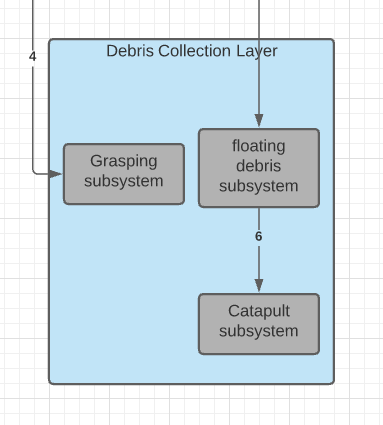
\includegraphics[width=0.60\textwidth]{images/subsystem_debris}
 \caption{Example subsystem description diagram}
\end{figure}

\subsubsection{Assumptions}
Since the debris collection is clearly spelled out in the competition instructions, no assumptions are necessary for this subsystem.

\subsubsection{Responsibilities}
Grab the underwater debris, be able to hold onto the debris while the submarine is navigating through water with water resistance pushing the block, and then release the debris in the deposit location.

\subsubsection{Subsystem Interfaces}

\begin {table}[H]
\caption {Subsystem interfaces} 
\begin{center}
    \begin{tabular}{ | p{1cm} | p{6cm} | p{3cm} | p{3cm} |}
    \hline
    ID & Description & Inputs & Outputs \\ \hline
    \#xx & Description of the interface/bus & \pbox{3cm}{input 1 \\ input 2} & \pbox{3cm}{output 1}  \\ \hline
    \#xx & Description of the interface/bus & \pbox{3cm}{N/A} & \pbox{3cm}{output 1}  \\ \hline
    \end{tabular}
\end{center}
\end{table}

\subsection{Subsystem 2 floating debris subsystem}
\subsubsection{Assumptions}
Since the debris collection is clearly spelled out in the competition instructions, no assumptions are necessary for this subsystem.

\subsubsection{Responsibilities}
collect debris floating on top of the water and deposit it in the catapult system. This will be done kinetically so there are no inputs to this mechanism.

\subsubsection{Subsystem Interfaces}

\begin {table}[H]
\caption {Subsystem interfaces} 
\begin{center}
	\begin{tabular}{ | p{1cm} | p{6cm} | p{3cm} | p{3cm} |}
		\hline
		ID & Description & Inputs & Outputs \\ \hline
		\#xx & Description of the interface/bus & \pbox{3cm}{input 1 \\ input 2} & \pbox{3cm}{output 1}  \\ \hline
		\#xx & Description of the interface/bus & \pbox{3cm}{N/A} & \pbox{3cm}{output 1}  \\ \hline
	\end{tabular}
\end{center}
\end{table}

\subsection{Subsystem 3}
\subsection{Subsystem 2 catapult subsystem}
\subsubsection{Assumptions}
We assumed it will be necessary to launch the debris up a little bit in order to get it over the lip of the deposit station.

\subsubsection{Responsibilities}
launch the floating debris that we collected into the deposit station.

\subsubsection{Subsystem Interfaces}

\begin {table}[H]
\caption {Subsystem interfaces} 
\begin{center}
	\begin{tabular}{ | p{1cm} | p{6cm} | p{3cm} | p{3cm} |}
		\hline
		ID & Description & Inputs & Outputs \\ \hline
		\#xx & Description of the interface/bus & \pbox{3cm}{input 1 \\ input 2} & \pbox{3cm}{output 1}  \\ \hline
		\#xx & Description of the interface/bus & \pbox{3cm}{N/A} & \pbox{3cm}{output 1}  \\ \hline
	\end{tabular}
\end{center}
\end{table}


\newpage

\section{Video Layer Subsystems}

\subsection{Subsystem 1 camera subsystem}
This section should be a general description of a particular subsystem for the given layer. For most subsystems, an extract of the architectural block diagram with data flows is useful. This should consist of the subsystem being described and those subsystems with which it communicates.

\begin{figure}[h!]
	\centering
 	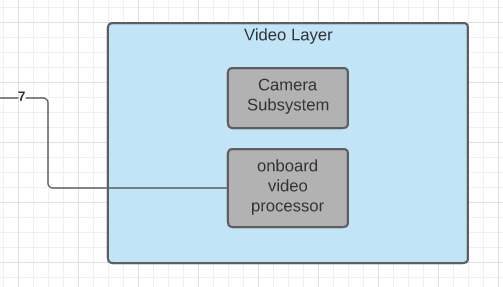
\includegraphics[width=0.60\textwidth]{images/subsystem_video}
 \caption{Example subsystem description diagram}
\end{figure}

\subsubsection{Assumptions}
We made the assumption that we would not be able to navigate the submarine without an underwater perspective.

\subsubsection{Responsibilities}
the responsibility of the camera is to capture the perspective of the submarine and relay it back to the video monitor.

\subsubsection{Subsystem Interfaces}
Each of the inputs and outputs for the subsystem are defined here. Create a table with an entry for each labelled interface that connects to this subsystem. For each entry, describe any incoming and outgoing data elements will pass through this interface.

\begin {table}[H]
\caption {Subsystem interfaces} 
\begin{center}
    \begin{tabular}{ | p{1cm} | p{6cm} | p{3cm} | p{3cm} |}
    \hline
    ID & Description & Inputs & Outputs \\ \hline
    \#xx & USB interface & \pbox{3cm}{USB } & \pbox{3cm}{USB port to Raspberri pi}  \\ \hline
    \end{tabular}
\end{center}
\end{table}

\subsection{Subsystem 2 onbaord video processor} 
\subsubsection{Assumptions}
We made the assumption that we the video will need to be relayed to some sort of small computer for processing and then sending on its way to our video monitor system.

\subsubsection{Responsibilities}
take the live USB feed of the video camera and propagate it back to our video monitor via the tether.

\subsubsection{Subsystem Interfaces}
\begin {table}[H]
\caption {Subsystem interfaces} 
\begin{center}
	\begin{tabular}{ | p{1cm} | p{6cm} | p{3cm} | p{3cm} |}
		\hline
		ID & Description & Inputs & Outputs \\ \hline
		\#xx & USB interface & \pbox{3cm}{USB } & \pbox{3cm}{Tether wire}  \\ \hline
	\end{tabular}
\end{center}
\end{table}



\newpage

%%% References
\bibliographystyle{plain}
\bibliographystyle{reference/IEEEtran_custom}
\bibliography{reference/refs}{}

\end{document}